\documentclass[10pt]{article}
\usepackage[a4paper,margin=0.85in]{geometry}
\usepackage{booktabs}
\usepackage{graphicx}
\usepackage{enumitem}
\usepackage{amsmath}
\usepackage[hidelinks]{hyperref}
\setlist{topsep=2pt,itemsep=1pt,parsep=0pt}
\setlength{\parindent}{0pt}
\setlength{\parskip}{4pt}
\title{\vspace{-1.5em}Data Analytics 1, Assignment 2, Part 2:\\BUC and Attribute-Oriented Induction on Census Data}
\author{}
\date{}
\begin{document}
\maketitle
\vspace{-3em}

\section*{1. Data and setup}
The dataset has 299,285 rows and 42 columns. The cube uses 12 raw categorical columns with no missing markers: \texttt{class\_of\_worker} (9 values), \texttt{education} (17), \texttt{marital\_status} (7), \texttt{industry\_code\_major} (24), \texttt{occupation\_code\_major} (15), \texttt{race} (5), \texttt{hispanic\_origin} (10), \texttt{sex} (2), \texttt{employment\_status} (8), \texttt{tax\_filer\_status} (6), \texttt{household\_summary} (8) and \texttt{citizenship} (5).
\texttt{instance\_weight} is excluded because it is a sampling weight, and \texttt{income} is the class label, so it is not a dimension. Duplicate rows are kept, so counts match the data as given. \texttt{NA} is a real value of \texttt{hispanic\_origin}, so the loader turns off pandas' default missing-value parsing.

\section*{2. BUC implementation}
\textbf{In-memory} (\texttt{buc\_memory.py}). \texttt{buc\_in\_memory(data, dims, minsup, out\_path, measure)} takes the dimension list, the measure and minsup. The measure is COUNT, or SUM of an integer column alongside the count. The iceberg test always uses COUNT. The recursion aggregates a partition, then for each later dimension splits it by value and recurses only into values that reach minsup. A partition below minsup cannot contain a cell that reaches it, so the branch is skipped. The split is a counting sort written with NumPy; no database or dataframe groupby takes part in the cube.

\textbf{Out-of-core} (\texttt{buc\_disk.py}). The memory budget in bytes is a parameter, and the relation is a file of fixed-width 20-byte records. A partition that fits the budget is loaded and finished by the in-memory recursion. A larger partition stays on disk:
\begin{enumerate}
\item One streaming pass gets its count, sum and a histogram of each remaining dimension.
\item Its cell is written.
\item For each remaining dimension, another pass distributes the rows of frequent values into one spill file per value, through bounded write buffers. This is the counting sort, done on disk.
\item Each spill file is processed recursively in ascending value order, then deleted.
\end{enumerate}
Cells leave in the same depth-first order in both versions, so their output files must be byte-identical, which is a stricter test than comparing sets of cells.

\section*{3. Verification}
Each setting below compared both versions with DuckDB, on \textbf{all 12 dimensions and all 4,096 group-bys}, cell by cell, for cell values, counts and sums. A single 12-column \texttt{CUBE} ran out of memory at DuckDB's 6.2 GB limit, so the reference runs as 16 batches: each fixes which of the first 4 dimensions are grouped and takes a \texttt{CUBE} of the other 8, with \texttt{HAVING COUNT(*) >= minsup}. Together these are exactly the same 4,096 group-bys.
\begin{center}\small
\begin{tabular}{rlrrrcc}
\toprule
minsup & Measure & Budget & Cells & Group-bys matching & Equal to DuckDB & Byte-identical \\
\midrule
1,000 & SUM(capital\_gains) & 1 MB & 143,132 & 4,096 / 4,096 & yes & yes \\
1,000 & COUNT only & 1 MB & 143,132 & 4,096 / 4,096 & yes & yes \\
200 & SUM(capital\_gains) & 4 MB & 657,012 & 4,096 / 4,096 & yes & yes \\
5,000 & SUM(capital\_gains) & 128 KB & 22,177 & 4,096 / 4,096 & yes & yes \\
\bottomrule
\end{tabular}
\end{center}
All 4,096 group-bys held at least one cell in every setting, so none passed trivially. At 128 KB every one of the 22,177 cells came from a disk partition, so the spill path alone produced that cube. Unit tests also compare both versions with a brute-force cube on small random data (6 tests pass).

\textbf{Does the budget hold?} \texttt{tracemalloc} measured the real allocations with only the record file as input:
\begin{center}\small
\begin{tabular}{rrr}
\toprule
Budget & Peak traced & Peak / budget \\
\midrule
256 KB & 249,801 B & 0.95 \\
1 MB & 956,179 B & 0.91 \\
4 MB & 3,669,303 B & 0.87 \\
\bottomrule
\end{tabular}
\end{center}
The budget bounds the buffers and arrays this code allocates, not the whole Python process: the interpreter and imported libraries take far more than 128 KB on their own.

The first version failed this check, at 1.7$\times$ the budget at 256 KB and 3.3$\times$ at 1 MB, while its output was correct. There were three causes: \texttt{tobytes()} copied each spill buffer when flushing; the per-row estimate left out the work array of NumPy's stable radix sort; and building spill file names with \texttt{pathlib} interned tens of thousands of unique strings, which grew Python's intern table by about 2 MB. All three were fixed. A correct result does not show that a memory limit is respected, so it had to be measured.

\section*{4. Performance analysis}
Each point is the median of 3 runs, with bars from the fastest to the slowest run. Experiments ran one at a time. The machine was a laptop on battery with antivirus active, and its speed changed between sessions by up to about 2$\times$: the same 143,132-cell run took 25 to 65 s. Repeats within a point usually agree closely, and the minsup sweep was rerun after its first point landed in a slow spell. \textbf{Compare points within a plot, not seconds across plots.}

\begin{center}
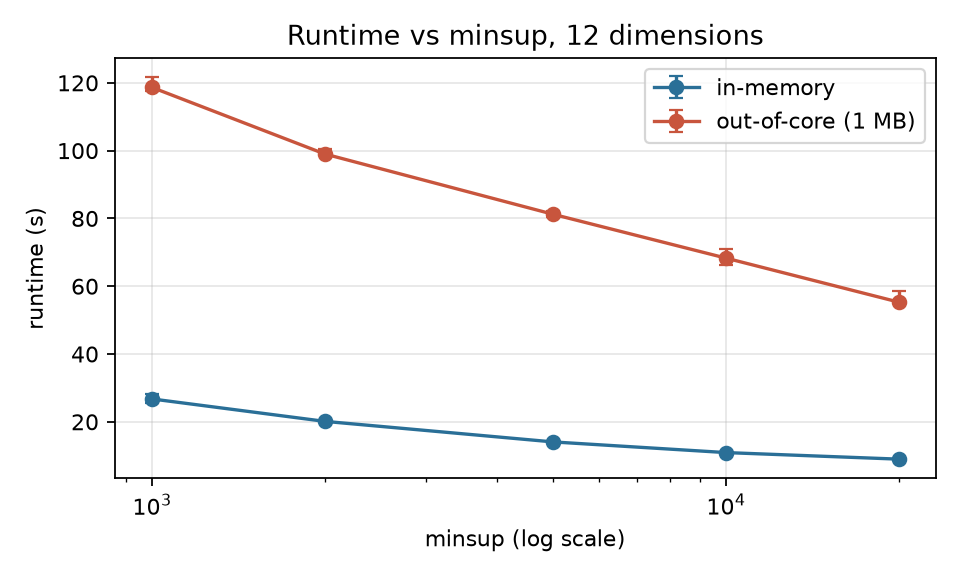
\includegraphics[width=0.48\textwidth]{../outputs/plots/minsup_runtime.png}
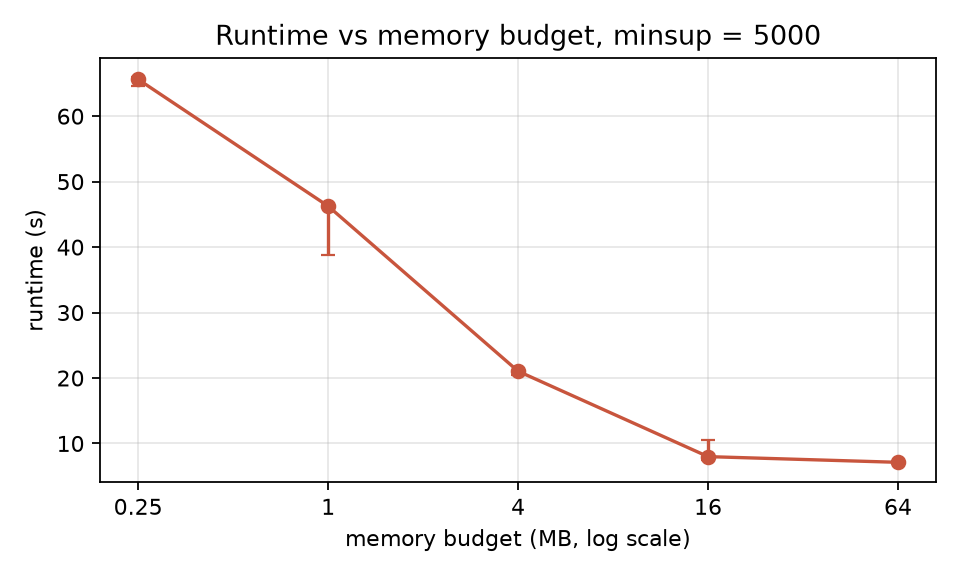
\includegraphics[width=0.48\textwidth]{../outputs/plots/memory_runtime.png}
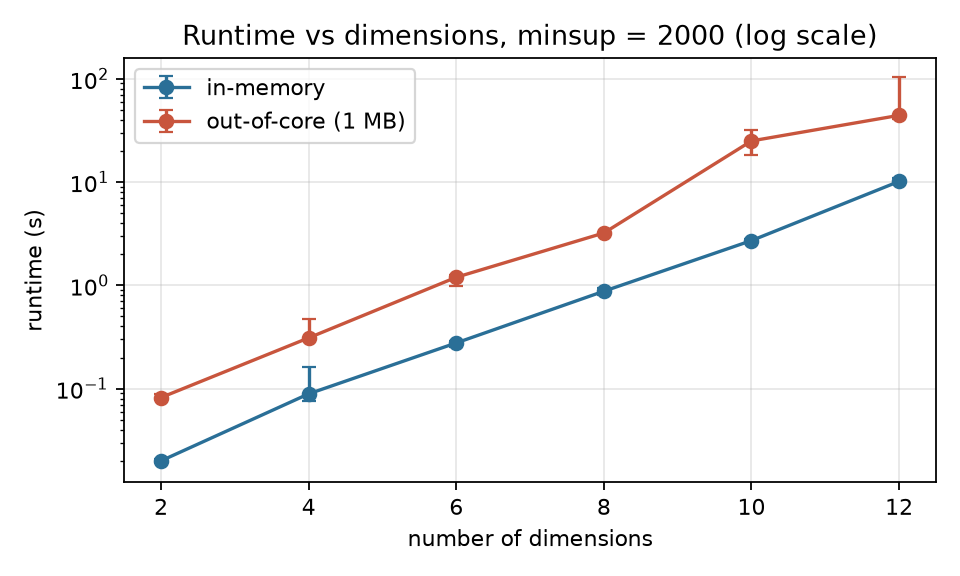
\includegraphics[width=0.48\textwidth]{../outputs/plots/dims_runtime.png}
\end{center}

\textbf{minsup vs runtime (memory fixed at 1 MB).} Raising minsup from 1,000 to 20,000 shrinks the cube 19$\times$ (143,132 to 7,360 cells) but cuts in-memory runtime only 3.0$\times$ (26.7 to 9.0 s) and out-of-core runtime 2.1$\times$ (118.7 to 55.3 s). Runtime does not follow cell count, because the upper levels of the recursion, which sort the large partitions, are needed at any minsup. The disk version barely changes its I/O: it reads 14.8 GB at minsup 1,000 and still 12.4 GB at 20,000, since the large partitions must be spilled either way. It runs 4 to 6$\times$ slower than in-memory.

\textbf{Memory vs runtime (minsup fixed at 5,000).}
\begin{center}\small
\begin{tabular}{rrrrr}
\toprule
Budget & Runtime (s) & Read (GB) & Disk partitions & Memory partitions \\
\midrule
256 KB & 65.6 & 17.6 & 22,177 & 0 \\
1 MB & 46.3 & 14.4 & 7,817 & 4,626 \\
4 MB & 21.0 & 5.1 & 543 & 2,510 \\
16 MB & 8.0 & 0.37 & 5 & 162 \\
64 MB & 7.1 & 0.006 & 0 & 1 \\
\bottomrule
\end{tabular}
\end{center}
This is the classic time-for-space trade. Runtime falls steeply until the budget is large enough for most partitions to load, then flattens: 16 MB is almost as fast as 64 MB, where the whole relation loads once and nothing spills. The 5.99 MB relation needs about 33 MB under the conservative per-row estimate of 110 bytes, which is why it fits only at 64 MB. Even at 256 KB, about 4\% of the relation's size, the cube is complete and matches. Peak spill space stayed at about 21 MB, 3.5$\times$ the relation.

\textbf{Dimensions vs runtime (minsup fixed at 2,000).} Cells grow from 46 at 2 dimensions to 67,215 at 12, and in-memory runtime from 0.02 to 10.1 s. From 8 dimensions on, each 2 extra dimensions multiply both cells and runtime by about 3 to 4$\times$, close to the 4$\times$ growth in the number of group-bys ($2^d$). Growth is therefore exponential in the number of dimensions even with pruning, and the log-scale plot is close to a straight line. The disk curve follows the same shape, with more spread at 10 and 12 dimensions (25.0 s with a range of 18 to 32 s at 10; one 103 s outlier at 12).

\section*{5. Optimization: dimension reordering}
\textbf{Idea.} BUC's cost depends on the order in which it processes dimensions. Taking a high-cardinality dimension first splits the data into small partitions early, so they fall below minsup sooner and whole branches are pruned. The optimised version sorts dimensions by descending cardinality. It changes no result, only the order of work.

\textbf{Benchmark.} Same input, minsup 2,000, 12 dimensions, 67,215 cells; 5 interleaved runs for the in-memory version and 3 for out-of-core. All five orders gave the identical cube after putting columns back in the same order. Some runs hit the slow state and took about 2$\times$ as long, so the fastest run is the more reliable column.
\begin{center}\small
\begin{tabular}{lrrrr}
\toprule
Order (in-memory) & Fastest (s) & Median (s) & Partition steps & Values pruned \\
\midrule
Given (unoptimised) & 10.21 & 11.20 & 72,669 & 305,572 \\
\textbf{Descending cardinality} & \textbf{9.45} & \textbf{10.69} & \textbf{71,146} & 186,444 \\
Ascending cardinality & 10.12 & 11.00 & 82,828 & 986,184 \\
Descending entropy & 11.45 & 20.77 & 71,662 & 319,905 \\
Ascending entropy & 10.60 & 11.12 & 82,771 & 1,016,300 \\
\bottomrule
\end{tabular}
\end{center}
\begin{center}
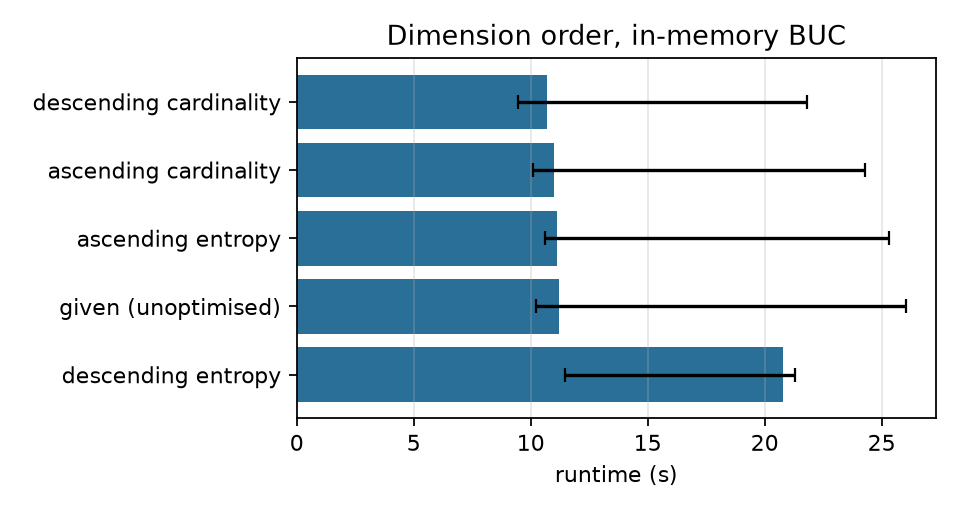
\includegraphics[width=0.6\textwidth]{../outputs/plots/order_runtime.png}
\end{center}
\textbf{Result.} Descending cardinality is the best order, but the in-memory gain is small: 7.5\% on the fastest run, 4.6\% on the median, and 2.1\% fewer partition steps. The descending-entropy median of 20.77 s comes from the slow state, not the order: its fastest run was 11.45 s. Entropy, which also accounts for skew, did not beat plain cardinality. The ascending orders do about 14\% more partition steps yet take similar time, which shows that the extra steps are on small, cheap partitions.

The gain is larger out of core: \textbf{100.0 s down to 87.8 s, a 1.14$\times$ speed-up}, probably because each pass over a large partition costs real I/O, so shrinking partitions early saves more. The gain is modest overall because the cost is dominated by the 67,215 cells that must be produced under any order. Reordering can only remove work on cells that fail minsup.

\section*{6. Attribute-Oriented Induction}
\textbf{Hierarchies} are stored as data in \texttt{hierarchies/}: age and weeks worked as ranges; education, class of worker, marital status, citizenship and race as hand-written trees; and industry and occupation as detail $\to$ major $\to$ sector.

\textbf{Method.} The relevant attributes are age, education, class of worker, marital status, occupation, industry, sex, weeks worked, country of birth and wage per hour. With an attribute threshold of 6, an attribute with too many values climbs its hierarchy, and it is removed if it has no higher level that fits. With a relation threshold of 80, the attribute with the most values then climbs until few enough tuples remain, and it is removed if it would reach ANY. Identical tuples are merged and counted. For the discriminant rules, both classes are generalised together to the same levels.

Weights follow Han and Kamber, for a generalised tuple $q$:
\[ t\text{-weight}(q) = \frac{\text{count}(q \in \text{target})}{\text{count}(\text{target})}, \qquad
d\text{-weight}(q) = \frac{\text{count}(q \in \text{target})}{\text{count}(q \in \text{target}) + \text{count}(q \in \text{contrast})} \]
A t-weight says how typical $q$ is of the target. A d-weight says how much of $q$ is target, so it must be read against the base rate: 18,568 of 299,285 rows, or 6.2\%.

\textbf{Attribute removal.} Country of birth and wage per hour have too many values and no hierarchy. Industry still has 8 sectors at its top level, above the threshold. Occupation was removed to meet the relation threshold.

\textbf{Characteristic rules for income $>$ \$50K} (79 rules, t-weights sum to 100\%; top rules, all with \texttt{class\_of\_worker} = Employed and \texttt{weeks\_worked} = Worked):
\begin{center}\small
\begin{tabular}{llllrr}
\toprule
Age & Education & Marital status & Sex & Count & t-weight \\
\midrule
35--64 & Degree & Ever married & Male & 7,082 & 38.14\% \\
35--64 & No degree & Ever married & Male & 3,447 & 18.56\% \\
35--64 & Degree & Ever married & Female & 1,772 & 9.54\% \\
Under 35 & Degree & Ever married & Male & 1,018 & 5.48\% \\
35--64 & No degree & Ever married & Female & 653 & 3.52\% \\
\bottomrule
\end{tabular}
\end{center}
The top three rules cover 66.25\% of high earners.

\textbf{Discriminant rules against income $\le$ \$50K} (32 tuples, 31 with target rows; age was removed here because the two classes together need more generalisation). Rules with at least 200 target rows, chosen to show both ends:
\begin{center}\small
\begin{tabular}{lllllrrrr}
\toprule
Education & Class & Marital status & Sex & Weeks & Target & Contrast & d-weight & Lift \\
\midrule
Degree & Employed & Ever married & Male & Worked & 8,441 & 11,499 & 42.33\% & 6.82 \\
Degree & Not employed & Ever married & Male & Worked & 228 & 676 & 25.22\% & 4.07 \\
Degree & Employed & Never married & Male & Worked & 715 & 4,216 & 14.50\% & 2.34 \\
Degree & Employed & Ever married & Female & Worked & 2,192 & 14,854 & 12.86\% & 2.07 \\
No degree & Employed & Ever married & Male & Worked & 4,204 & 32,059 & 11.59\% & 1.87 \\
No degree & Employed & Ever married & Female & Worked & 789 & 33,040 & 2.33\% & 0.38 \\
\bottomrule
\end{tabular}
\end{center}
Lift is the d-weight divided by the 6.2\% base rate. The pattern is clear: a degree helps at every level, and the same profile with \texttt{sex} = Female has a far lower d-weight (12.86\% against 42.33\%). This describes the sample, unweighted by \texttt{instance\_weight}, and it is an association, not a cause.

\textbf{Children in the contrast class.} The contrast class contains 83,709 people under 18, almost none of whom can earn over \$50K. Limiting both classes to adults raises the base rate from 6.20\% to 8.61\%. The top rule's d-weight stays at 42.33\%, because no adult profile changes much, but its lift falls from 6.82 to 4.92. Lift from the full data overstates how distinctive these profiles are among adults.

\textbf{Checking the generalisation code.} The real \texttt{generalize} function was run on the four detail/summary pairs in the data. Tables were learned from a random half of the rows and tested on the other half:
\begin{center}\small
\begin{tabular}{lrrl}
\toprule
Pair & Rows tested & Match & Exceptions \\
\midrule
Industry detail $\to$ major & 149,643 & 100\% & none \\
Occupation detail $\to$ major & 149,643 & 100\% & none \\
Household status $\to$ summary & 149,640 & 99.97\% & \texttt{In group quarters} has several parents \\
State $\to$ region & 149,643 & 99.81\% & \texttt{?} and \texttt{Abroad} have several parents \\
\bottomrule
\end{tabular}
\end{center}
All mismatches come from the values that have more than one parent in the data, so the code is correct. Three further household rows have a value that was never seen in the learning half.

\textbf{The data's region column is not real geography.} A hand-written table of the US Census regions disagrees with the data for 28 states, for example Michigan is labelled Northeast, Utah South and New York West. Each state maps consistently, so the pair behaves like a hierarchy, but among rows with a named state only 9,742 of 21,493 agree with the Census. Region of previous residence should not be read as geography in this dataset.

\textbf{Sensitivity.} The relation threshold controls output size directly: thresholds of 5, 20, 50, 100 and 200 give 4, 16, 31, 79 and 186 rules, with 2, 4, 5, 6 and 6 attributes kept.

\textbf{Cross-check with BUC.} AOI's generalised relation is the base cuboid of a cube on the generalised attributes. Running BUC at minsup 1 on those 6 attributes gave 935 cells, of which 79 are at the base level, and their counts are identical to the 79 AOI tuples.

\section*{7. Comparison of BUC and AOI}
\begin{center}\small
\begin{tabular}{p{0.2\textwidth}p{0.36\textwidth}p{0.36\textwidth}}
\toprule
 & \textbf{BUC} & \textbf{AOI} \\
\midrule
Purpose & Precompute every frequent aggregate, exactly & Summarise a class in a few general statements \\
Question answered & ``How many rows have these exact values?'' & ``What does this class look like, and what sets it apart?'' \\
Best at finding & Exact frequent combinations, for OLAP slicing & Typical and distinguishing profiles \\
Output here & 143,132 cells at minsup 1,000 & 79 characteristic rules; 32 discriminant tuples \\
Output size set by & minsup, indirectly & Thresholds, directly \\
Needs domain knowledge & No & Yes: concept hierarchies \\
Detail & Keeps exact values; loses nothing that is frequent & Trades detail for readability \\
Cost & Exponential in dimensions: 26.7 s at 12 dimensions, minsup 1,000 & Under 2 s for characteristic rules \\
Scale & Has an out-of-core version here; verified at 128 KB & In memory here; one pass per climb \\
\bottomrule
\end{tabular}
\end{center}

\textbf{Interpretability.} AOI's top rule can be read aloud: 38.14\% of high earners are employed, ever-married men aged 35--64 with a degree who worked during the year. BUC holds the same facts across thousands of cells, and a reader has to query them.

\textbf{Efficiency.} The times are not a like-for-like race, because the two methods do different jobs. On the same 6 generalised attributes, BUC took 0.06 s for 935 cells, because generalisation had already shrunk the problem. The discriminant run took longer than the characteristic run (41.7 s against 1.8 s) because it works on all 299,285 rows rather than the 18,568 target rows, and each climb merges them again.

\textbf{They are connected.} The cross-check above shows that AOI's output is the base cuboid of a cube on generalised attributes. AOI chooses a level of detail; BUC then enumerates every aggregate at that level.

\textbf{When to prefer each.}
\begin{itemize}
\item \textbf{BUC:} for a dashboard or OLAP tool that needs fast exact answers, such as how many self-employed women hold a doctorate, or when the questions are not known in advance.
\item \textbf{AOI:} for explaining a group to a person, such as a short profile of high earners, when good hierarchies exist.
\item \textbf{Both:} use AOI to find a profile, then BUC cells to drill into exact counts behind it.
\end{itemize}

\textbf{A limit of AOI seen here.} The ``climb the attribute with the most values'' rule is blind to usefulness: with a tight threshold it removed occupation, and in the discriminant run age, both of which plainly relate to income. The attribute list and thresholds therefore need human judgement.
\end{document}
